\documentclass{article}
\title{Too good to be true: Underdispersion in geochronology}
\author{}
\date{}
\usepackage{graphicx,fullpage,natbib,amsmath,caption}
\usepackage[colorlinks=true, urlcolor=black, linkcolor=black, citecolor=black]{hyperref}
\usepackage{lineno}
\linenumbers
\begin{document}

\maketitle
\vspace{-3em}

\begin{abstract}
Statistical hypothesis testing is widely used in geochronology to
assess whether multiple analyses of a sample are consistent with a
single age. Failure of such tests is evidence for excess scatter
(`overdispersion'), suggesting geological complexity or faulty
data. In contrast, this paper highlights the opposite and largely
overlooked problem of `underdispersion', in which datasets agree
unrealistically well with the null hypothesis and appear `too good to
be true'. Underdispersion can arise from incorrect propagation of
analytical uncertainties or from over‑zealous outlier rejection that
inflates p‑values and suppresses genuine geological
variability.\medskip

This paper introduces a simple graphical diagnostic for identifying
systematic underdispersion across collections of geochronological
studies, based on the empirical cumulative distribution of p‑values
from chi‑squared tests of data homogeneity.  While overdispersion
shifts p‑value distributions above and to the left of the 1:1 line in
cumulative probability space, there are no natural mechanisms that
should produce an excess of very high p‑values.  The area below the
1:1 line in a cumulative probability plot defines a `forbidden zone'
and provides a meta-analytical signature of underdispersion.\medskip

The proposed method is demonstrated using synthetic examples and
applied to extensive compilations of published geochronological data,
including fission‑track analyses, mass‑spectrometer‑based chronometers
reported in high‑profile journals, datasets underlying the geologic
time scale, and detrital zircon U--Pb age spectra.  These case studies
reveal widespread and sometimes extreme underdispersion, particularly
in fission‑track data and $^{40}$Ar/$^{39}$Ar age plateaux, at levels that
cannot be explained by chance alone.\medskip

Underdispersion matters because it creates unwarranted confidence in
apparently precise ages at the expense of accuracy and obscures
meaningful geological information carried by excess scatter.  The
diagnostic plot introduced here provides a practical step towards
recognising when data have been over‑processed, and towards restoring
a more balanced treatment of dispersion in geochronology.
\end{abstract}

\section{Introduction}\label{sec:intro}

The scientific method is a uniquely powerful tool for discovery and
objective decision-making \citep{popper1959}. Statistical hypothesis
testing is often used to formalise this process. If an observed
experimental result is unlikely under a mathematically defined null
hypothesis, the hypothesis is rejected; otherwise, it is retained
(Section~\ref{sec:definitions}).  When used correctly, hypothesis
tests are extremely valuable. For instance, powered tests in
double-blind clinical trials form the foundation of the pharmaceutical
drug approval process\footnote{A powered test specifies in advance the
sample size needed to detect a particular effect -- for example, a
50\% reduction in mortality}.  In this way, hypothesis testing can
literally save lives. However, unpowered tests are vulnerable to both
conscious and unconscious misuse.\medskip

Formalised hypothesis tests create an artificial dichotomy between
results that support or reject scientific hypotheses. This binary
thinking introduces bias into research findings. Arbitrary p-value
cutoffs (typically at $\alpha = 0.05$) incentivise researchers to bias
data to fit one side of the divide \citep{amrhein2019}. When an entire
community of scientists tries to reject a statistical hypothesis, it
increases the risk of committing a so-called Type~I error (false
positive). This is a serious issue in the life sciences, which may
even cause most published research findings to be false
\citep{ioannidis2005}.\medskip

This paper will show that geochronology experiences the opposite
problem, whereby hypothesis tests are exclusively used to check
whether a dataset is `simple' before proceeding with another
statistical procedure \citep{mcintyre1966}. In geochronology, failure
of the test indicates the presence of excess scatter
(`overdispersion'), which may be diagnostic of faulty data or
geological complexity (Section~\ref{sec:overdispersion}).  Removal of
perceived `outliers' avoids this complexity and makes life
considerably easier. However, taking this approach too far can lead to
Type~II errors (false negative) and, in the most extreme cases, to
`underdispersed' datasets that are `too good to be true'
(Section~\ref{sec:causes}).\medskip

Geochronologists are increasingly aware of these issues. Over the past
decade, several papers and community recommendations have appeared,
discussing the geological causes of overdispersion and introducing new
statistical strategies to avoid over-zealous outlier detection
\citep[e.g.,][]{horstwood2016,keller2018,klein2024,vermeesch2025c}.
Nevertheless, underdispersed datasets are still more likely to pass
through peer review than overdispersed datasets, providing an
incentive to `clean up' datasets.\medskip

A key challenge is that there is currently no clear definition of
underdispersion, nor a straightforward way to detect it. This paper
addresses that gap by introducing a simple graphical method for
identifying underdispersion in geochronological datasets
(Section~\ref{sec:ecdf}). The method is demonstrated using both
synthetic (Section~\ref{sec:synthetic}) and real datasets
(Section~\ref{sec:real}) to evaluate how common underdispersion is in
the published literature. Providing an accessible diagnostic tool is
an important first step toward solving the problem.

\section{Definitions}\label{sec:definitions}

Rare exceptions notwithstanding, most radiometric age estimates are
based on multiple analyses (aliquots) per sample.  This redundancy
of measurements benefits the precision of the age estimates (which
scales with the inverse of the square root of the number of analyses)
and provides an opportunity to assess the internal consistency of the
data. In statistics, it is useful to make a distinction between the
true values and their statistical estimates, where

\begin{enumerate}
\item The true values could be the actual \emph{ages} of some minerals
  separated from a rock sample and the estimates are \emph{dates} with
  some analytical uncertainty; or
\item The true values could be a pair of
  \textsuperscript{206}Pb/\textsuperscript{238}U and
  \textsuperscript{207}Pb/\textsuperscript{235}U ratios which may or
  may not be concordant, and the estimated values are displaced from
  those true values by some random distance; or
\item The true values could be pairs of isotopic ratios that fall on a
  mixing line between radiogenic and non-radiogenic end-member
  components, and the estimate are offset from this mixing line,
  forming an isochron that can be fit by weighted least squares
  regression.
\end{enumerate}

The difference between the true and estimated values is the result of
two contributions:

\begin{enumerate}
\item Analytical uncertainty, which can be estimated from the raw mass
  spectrometer data by error propagation.
\item Geological scatter between the true values.
\end{enumerate}

The relative contributions between these two sources of dispersion can
be formally tested by formulating a null hypothesis $H_0$ and an
alternative hypothesis $H_a$:

\begin{description}
\item{$H_0$:} All the ages are the same.
\item{$H_a$:} Some ages are different.
\end{description}

The dispersion of the estimated values around the best fitting
weighted mean, concordia age or isochron can be quantified using the
error-weighted sum of the squared differences, $\chi^2$.  Under $H_0$,
$\chi^2$ follows a chi-squared distribution with $\nu$ \emph{degrees
of freedom}, where $\nu = 1$ for U--Pb concordance, $\nu = n-1$ for
weighted means, $\nu = n-2$ for two-dimensional isochrons and $\nu =
2\,n - 4$ for three-dimensional isochrons. This leads to three
equivalent ways to evaluate $H_0$:

\begin{enumerate}
\item High values of $\chi^2$ lead to the rejection of $H_0$ in favour of
  $H_a$.  The cutoff value $X_c^2$ corresponds to the $1-\alpha$
  quantile of the null distribution, where $\alpha$ is typically taken
  to be 5\% \citep{pearson1900};
\item The probability of observing a value exceeding $\chi^2$ under $H_0$
  is known as the \emph{p-value} of the chi-square test. P-values
  below $\alpha$ lead to the rejection of $H_0$;
\item The mean squared weighted deviation (MSWD) is defined as
  $\chi^2/\nu$.  If $H_0$, is true and $\nu>20$, then the null
  distribution of the MSWD is approximately Gaussian with a mean of
  $\sim\,1$ and a standard deviation $\sqrt{2/\nu}$. MSWD values fall
  outside the range of $1 \pm 2\,\sqrt{2/\nu}$ lead to the rejection
  of $H_0$ \citep{wendt1991}.
\end{enumerate}

Datasets for which $\chi^2 > X_c^2$, $p < \alpha$ or
MSWD$\,>1+2\,\sqrt{2/\nu}$ are said to be \emph{overdispersed} with
respect to the analytical uncertainties. Dataset for which
$\chi^2 \approx 0$, $p > 1-\alpha$ and MSWD$\,<1-2\,\sqrt{2/\nu}$ are
\emph{underdispersed}.

\section{What causes overdispersion?}\label{sec:overdispersion}

As explained in Section~\ref{sec:definitions}, overdispersion is the
phenomenon whereby the observed scatter of the measurements around the
mean or isochron exceeds the range expected from the analytical
uncertainties alone. This leads to the rejection of $H_0$ in favour of
$H_a$, which can mean four things:

\begin{enumerate}
\item The analytical uncertainties have been underestimated;
\item Something has gone wrong during the sample preparation or
  analysis, causing poor reproducibility of the measurements;
\item The true values are dispersed due to geological or
  sample-specific complexities that are not captured by the analytical
  uncertainties;
\item The dataset has been cherry picked among a larger collection of
  measurements to maximise the dispersion. This situation never occurs
  in geochronology but is actually quite common in other fields of
  science as detailed in the Appendix (`Type~I cherry picking').
\end{enumerate}

Overdispersion carries a distinctly negative connotation in
geochronology. For example, overdispersed isochrons are known as
`errorchrons' \citep{brooks1972}, reflecting the concern that weighted
least squares regression cannot safely be applied to datasets that
exhibit excess scatter around the best fit line. However, this
negative reputation is undeserved. If the first two scenarios can be
ruled out, the presence of overdispersion provides an opportunity to
extract additional information about the geological system of
interest.\medskip

Geological sources of overdispersion include protracted residence
times of datable minerals in magmatic systems, slow cooling of
minerals with variable closure temperatures, the presence of
xenocrysts or common Pb, and the occurrence of Pb-loss
\citep{galbraith1993,rioux2012,keller2018,klein2024}.\medskip

The statistical \emph{power} of the chi-squared test to detect
overdispersion steadily grows with increasing analytical precision and
sample size. Given a large enough sample with sufficiently small
analytical uncertainties, even the smallest amounts of geological
dispersion become discoverable.  Given the spectacular gains in
precision and throughput that radiometric geochronology has witnessed
over time, it is not surprising that overdispersed datasets become
ever more prevalent. Therefore, overdispersed datasets should be
expected to be the rule, not the exception \citep{vermeesch2025c}.

\section{What causes underdispersion?}\label{sec:causes}

Underdispersion is the phenomenon whereby the measured values cluster
together closer than expected from the analytical uncertainties.  This
may mean two things:

\begin{enumerate}
  \item The analytical uncertainties have been overestimated. This can
    happen when systematic sources of uncertainty are mistakenly
    treated as random uncertainties. Consider, for example, an
    LA-ICP-MS session in which instrument drift and elemental
    fractionation are estimated by analysing reference materials
    interspersed between the samples. Then it seems logical to add the
    internal reproducibility of the reference materials to the
    analytical uncertainties of the samples, in quadrature. However,
    doing so potentially introduces strong error correlations between
    the different aliquots of the sample, which may result in
    overestimated uncertainties \citep{mclean2016}.
  \item The data have been subjected to over-zealous `outlier
    detection' in order to remove values that are perceived to be in
    disagreement with $H_0$. A famous example of this type of
    behaviour is Gregor Mendel's study of the genetic traits of garden
    peas \citep{mendel1866}. A re-analysis of Mendel's data by
    \citet{fisher1936} using the chi-squared test yielded a p-value of
    0.99993, which is `too good to be true'. In this paper, we will
    refer to this type of behaviour as `Type~II cherry picking', for
    reasons that are provided in the Appendix. Mendel's motivations
    for Type~II cherry picking have been discussed at length in the
    literature \citep{radick2015}. Whatever they may have been in
    1866, it should be clear that this type of data manipulation has no
    place in modern science.
\end{enumerate}

In the case of Mendel's experiment, a single p-value sufficed to
identify the cherry picking. Such extreme cases of underdispersion are
rare in geochronology, although they do exist. In most cases,
underdisperseion is more subtle, as an unintentional consequence of
outlier detection. For example, when constraining the eruption age of
a volcanic tuff from zircon U--Pb dates, it is common practice to
remove antecrystic `outliers' until the MSWD approaches unity. In the
case of plateau ages in Ar--Ar geochronology, some definitions of a
`plateau' even include an explicit p-value criterion
\citep{jourdan2009}.\medskip

These more subtle cases of underdispersion cannot be identified in a
single sample. For example, a p-value of 0.98 or greater has a chance
of 1 in 50 to occur by accident (no cherry picking) in datasets that
do not exhibit overdispersion. However, when such moderately high
p-values are systematically overrepresented in the literature, their
collective effect can be as clear as that of a single, strongly
underdispersed dataset. Section~\ref{sec:ecdf} presents some numerical
and graphical methods to detect this problem.

\section{A graphical means of detecting underdispersion}\label{sec:ecdf}

Assuming $n$ independent experiments, the probability that all $n$
p-values are at least $\alpha$ is $(1-\alpha)^n$.  Consequently, the
probability of making at least one Type~I error (i.e., incorrectly
classifying a homogeneous sample as overdispersed) is $1 - (1 -
\alpha)^n$. This probability increases from 5\% for $n = 1$, to 10\%
for $n = 2$, 14\% for $n = 3$, and 51\% for $n = 14$. In other words,
in geochronological studies of homogeneous samples reporting 14 or
more MSWD values, it becomes more likely than not that at least one
sample will be falsely identified as overdispersed.\medskip

The same reasoning can be applied to the lower tail of the chi-squared
distribution. For a non-dispersed sample, the probability of obtaining
a p-value greater than 0.5 is 50\%. For $n$ independent samples, the
probability that all p-values exceed 0.5 is
$2^{-n}$. Section~\ref{sec:real} will show that some published
datasets contain up to $n = 9$ p-values greater than 0.5. The
probability of such an outcome is less than 0.2\%. While this could
occur by chance within a large collection of studies, the repeated
occurrence of such uniformly high p-values is unlikely to be
coincidental and cannot reasonably be attributed to random variation
alone.\medskip

These simple calculations are informative but have important
limitations. They apply only to independent datasets evaluated at a
single, arbitrarily chosen p-value threshold, and they assume that all
samples have non-dispersed true isotopic ratios. However, in practice
the scientific literature comprises a heterogeneous mix of datasets in
which some samples exhibit varying degrees of overdispersion, some
studies may have applied various levels of outlier rejection, and many
studies may have sample sizes too small to determine conclusively
whether the deata are significantly underdispersed. A broader approach is
therefore required to identify underdispersion at scale. This paper
introduces a graphical method designed to detect underdispersion
across a collection of multiple studies.\medskip

Consider a representative collection of statistical hypothesis tests
extracted from the scientific literature. If \emph{all} the null
hypotheses for these tests are true then, by definition, the frequency
distribution of their p-values should follow a uniform
distribution. That is, 90\% of the p-values should be less than 0.9,
5\% of the p-values should be less than 0.05 and so forth.  The
empirical cumulative distribution function (ECDF) of such a set of
experimental outcomes would straddle the 1:1 line.  If \emph{some} of
the null hypotheses are false, then this would shift the p-value
distribution to the left and move its ECDF above the 1:1 line (blue
line in Figure~\ref{fig:ECDF}). The area below the 1:1 line is a
`forbidden zone', indicating an over-supply of high p-values.\medskip

There are no natural mechanisms that can push the p-value distribution
in the `forbidden zone'.  The only two mechanisms that can cause
underdispersed datasets are given in Section~\ref{sec:causes}: (1)
incorrect error propagation; and (2) removal of perceived `outliers'
to inflate the p-value. If the first mechanism can be ruled out, then
the p-value distribution can be used to detect systematic
underdispersion in the scientific literature.  Note that the ECDF of
the p-values can only be used to detect excessive outlier detection
(Type~II cherry picking, see Appendix).  Type~I cherry picking shifts
the p-value distribution towards the left and above the 1:1 line,
where genuinely false null hypotheses are also found.

\noindent\begin{minipage}[t][][b]{.5\linewidth}
  \includegraphics[width=\linewidth]{../figures/synthetic-ECDF.pdf}
\end{minipage}
\begin{minipage}[t][][t]{.5\linewidth}
  \captionof{figure}{p-value distribution using synthetic data,
    assuming correctly estimated analytical uncertainties. The blue
    curve shows the empirical cumulative distribution function (ECDF)
    of 100 simulated p-values derived from overdispersed samples. The
    red curve shows the ECDF of another set of 100 simulated p-values
    drawn from the same distribution, but with half of the samples
    affected by excessive outlier rejection.}
  \label{fig:ECDF}
\end{minipage}

\section{Synthetic examples}\label{sec:synthetic}

This section demonstrates the usefulness of the p-value distribution
as a diagnostic tool, using synthetic examples to illustrate the
different mechanisms that can give rise to underdispersion.

\subsection{Fission tracks}\label{sec:synthetic-FT}

Section~\ref{sec:causes} identified two mechanisms that can lead to
underdispersion: (1) incorrect error propagation and (2) overly
aggressive outlier rejection. Without fully transparent
data-processing pipelines, it is impossible to distinguish between
these causes. The only geochronological method with completely
transparent error propagation is the fission-track method using the
external detector approach \citep{hurford1983}.\medskip

For this type of data, the raw observations consist of paired
measurements of spontaneous and induced track counts, obtained by
human observers \citep[or by computer algorithms trained by human
  observers;][]{nachtergaele2021,boone2025}. The precision of the
fission track age estimates is entirely determined by these two
values, so that $s[N_s/N_i] = (N_s/N_i) \sqrt{1/N_s+1/N_i}$
\citep{galbraith1981}. Because $N_s$ and $N_i$ are typically small
(generally fewer than 100 and often fewer than 10), the precision of
single-grain fission track age estimates is usually low compared to
that of other (mass spectrometer-based) geochronometers. To improve
precision, it is customary to analyse multiple grains (typically
$n=20$) per sample and to average or pool their counts.\medskip

Before pooling multiple fission track measurements and treating them
as single grain, it is important to verify that the data are
homogeneous---that is, consistent with a single true age. This can be
assessed with the following test statistic:

\begin{equation}
  \chi^2 = \dfrac{1}{N_{s\ast}\,N_{i\ast}}
  \sum\limits_{j=1}^{n}\dfrac{\left(N_{sj}\,N_{i\ast}-N_{ij}\,N_{s\ast}\right)^2}
             {N_{sj}-N_{ij}}
\end{equation}

\noindent where $N_{sj}$ and $N_{ij}$ represent the
$j$\textsuperscript{th} (out of $n$) $N_s$ and $N_i$ values,
$N_{s\ast}\equiv\sum_{j=1}^nN_{sj}$ and
$N_{i,\ast}\equiv\sum_{j=1}^nN_{ij}$. Under $H_0$, this definition of
$\chi^2$ follows a chi-squared distribution with $n-1$ degrees of
freedom \citep{galbraith1993}.\medskip

Because fission track analysis is performed by human observers,
analysts must take particular care to avoid bias. Various strategies
can be used to minimise this risk. Arguably the most robust approach
for acquiring external detector data is to count spontaneous and
induced fission tracks separately (pers. comm., R.A.~Donelick). Under
this procedure, a set of $n$ grains is counted first, followed by
their corresponding $n$ mica images (or \emph{vice versa}). This
results in the following sequence of measurements: $N_{s1}, N_{s2},
\ldots, N_{sn}$, $N_{i1}, N_{i2}, \ldots, N_{in}$.\medskip

This `block counting' design minimises the risk of unconscious bias,
particularly when samples are analysed blindly, i.e. without the
analyst knowing the origin or even the name of the sample being
counted. Although this approach is used in some studies, most
laboratories adopt a different procedure in which the analyst
alternates between grains and mica images. This produces an
`interleaved' sequence of measurements: $N_{s1}, N_{i1}, N_{s2},
N_{i2}, \ldots, N_{sn}, N_{in}$.\medskip

This interleaving pattern is not always chosen by the analyst; it may
be imposed by the data acquisition software. A potential drawback of
this design is that it may lead analysts to consciously or
subconsciously converge on a particular $N_s/N_i$ ratio. Once the
first pair of track counts has been obtained, the analyst effectively
`knows' the result, which may influence the selection criteria for
subsequent grains. This type of behaviour can be simulated as follows:

\begin{enumerate}
\item Generate $n$ random values $r_j$ from a lognormal distribution
  with location parameter $\mu$ and dispersion parameter $\sigma$;
\item Generate $n$ pairs of $N_{sj}$ and $N_{ij}$ values from binomial
  distributions with parameters $\theta_j = r_j/(1+r_j)$ and sample
  sizes $N_j = N_{sj} + N_{ij}$, where $N_j$ is a random integer;
\item For $j=1\rightarrow{n}$, perform a chi-squared test on the first
  $j$ pairs of $N_s$ and $N_i$ values. If the test fails, adjust
  $N_{sj}$ and $N_{ij}$ until it passes, then proceed.
\end{enumerate}

The results of this numerical simulation are shown in
Figure~\ref{fig:FT}. It is important to note that observer drift is
only one possible mechanism for underdispersion, assuming that the
bias arises during fission track analysis. Alternative (or additional)
biases may occur \emph{post hoc}, through adjustments to fission track
counts after the original data acquisition. This second type of bias
affects block counting method and interleaved experimental design
equally and is analogous to the bias that can arise when removing
outliers from weighted means, as discussed in
Section~\ref{sec:weighted-mean}.

\noindent\begin{minipage}[t][][b]{.5\linewidth}
  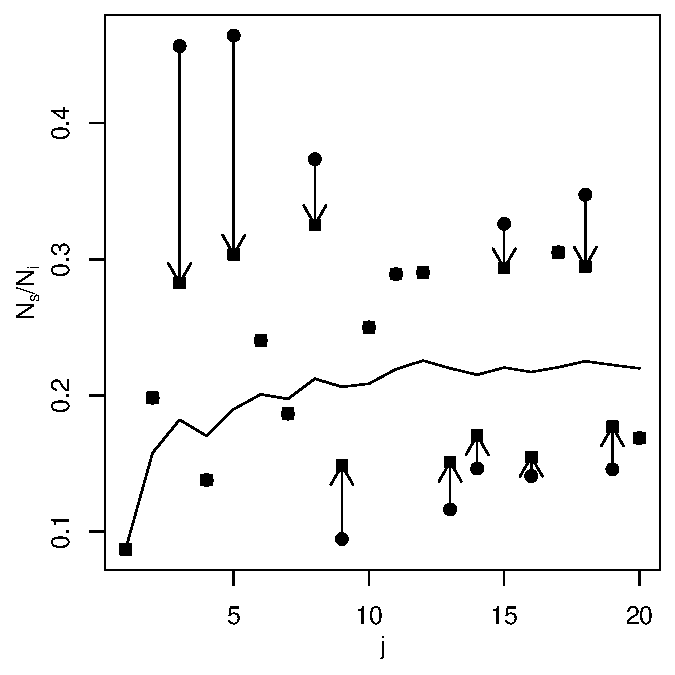
\includegraphics[width=\linewidth]{../figures/FT.pdf}
\end{minipage}
\begin{minipage}[t][][t]{.5\linewidth}
  \captionof{figure}{ Simulation of `observer drift' in fission track
    analysis. Circles are synthetic fission track ratios, drawn from a
    population with 20\% overdispersion. Black squares are adjusted
    values, ensuring that $p > 0.05$ for all counts up to and
    including $j$ (with $1\leq{j}\leq{n=20}$). The black line shows
    the pooled ratio for all counts up to and including $j$.}
  \label{fig:FT}
\end{minipage}

\subsection{Weighted means}\label{sec:weighted-mean}

Consider a collection of $n$ zircon crystals, which all formed at
exactly the same time, $t$. Suppose that the zircon crystals were
dated by the U--Pb method, yielding $n$ dates $\hat{t}_i$ with
analytical uncertainties $s[\hat{t}_i]$ (for $1\leq{i}\leq{n}$).
Then a precise estimate for $t$ can be obtained by taking the
weighted mean of the $n$ zircon dates:

\begin{equation}
  \bar{t} = \dfrac{\sum_{i=1}^{n}\hat{t}_i/s[\hat{t}_i]^2}
      {\sum_{i=1}^{n}1/s[\hat{t}_i]^2}
\end{equation}

The accuracy of this formula hinges on the assumption that the true
ages of all the zircon grains are identical. This assumption can be
tested by redefining the chi-square statistic:

\begin{equation}
  \chi^2 = \dfrac{1}{n-1}
  \sum\limits_{i=1}^n \left(\dfrac{\hat{t}_i-\bar{t}}{s[\hat{t}_i]}\right)^2
\end{equation}

Small values of $\chi^2$ indicate good agreement with the hypothesis
that all ages are identical, whereas large values suggest that this
assumption is less likely to hold. Several mechanisms can lead to this
outcome, including (1) the presence of xenocrysts, (2) common Pb, (3)
Pb-loss, and (4) genuine outliers. Failure of the chi-squared test
requires that the assumption of age homogeneity be dropped in favour
of a more complex model that captures these scenarios. If one is
willing to make the assumption that the dispersion is entirely caused
by genuine outliers, then the dataset can be trimmed until the dataset
passes the chi-squared test. This procedure can be simulated as
follows:

\begin{enumerate}
  \item\label{it:X2full} Calculate the p-value for the full dataset of
    $n$ dates.
  \item For $i=1\rightarrow{n}$, leave out the $i$\textsuperscript{th}
    measurement and calculate the p-value for the remaining $n-1$
    analyses; call these values $p_i$;
  \item\label{it:remove_outlier} Identify the aliquot with the highest
    value of $p_i$, and permanently remove it from the dataset;
  \item Recursively repeat
    steps~\ref{it:X2full}--\ref{it:remove_outlier} for the surviving
    dates until the dataset no longer fails the chi-squared test.
\end{enumerate}

This procedure is illustrated in Figure~\ref{fig:synthetic_U-Pb} using
a synthetic but realistic zircon U--Pb age distribution that includes
both young and old tails.

\noindent\begin{minipage}[t][][b]{.6\linewidth}
  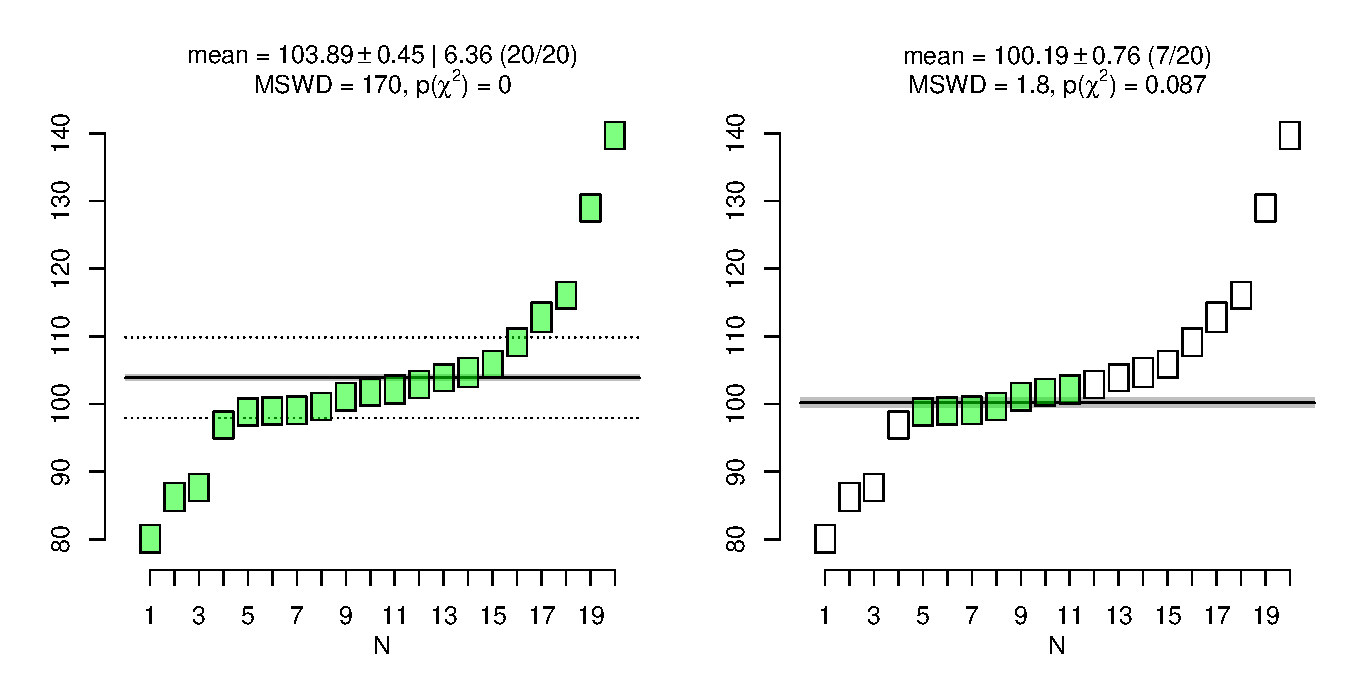
\includegraphics[width=\linewidth]{../figures/wtdmean.pdf}
\end{minipage}
\begin{minipage}[t][][t]{.4\linewidth}
  \captionof{figure}{Synthetic U--Pb dataset, comprised of a
    three-component mixture of (1) normally distributed ages with a
    mean $\mu_1 = 100$\,Ma and standard deviation $\sigma_1 = 5$\,Ma;
    (2) a positively truncated normal distribution of antecryst ages
    with mean $\mu_2 = \mu_1$ and standard deviation $\sigma_2 =
    20$\,Ma; and (3) a negatively truncated normal distribution of
    ages affected by Pb-loss, with mean $\mu_3 = \mu_1$ and standard
    deviation $\sigma_3 = 20$\,Ma. a) calculates the weighted mean
    including all aliquots; b) calculates the weighted mean with
    `outliers' removed until $p(\chi^2) > \alpha$.}
  \label{fig:synthetic_U-Pb}
\end{minipage}

\subsection{Isochrons}

Most mass-spectrometer based geochronometers are based on the
radioactive decay of a parent nuclide $P$ to a daughter nuclide $D$ in
the presence of a non-radiogenic `sister' isotope $d$. In general, $D$
consists of a mixture of radiogenic and non-radiogenic components,
whose relative contributions can be estimated by analysing multiple
cogenetic aliquots and fitting a straight line through their isotopic
ratios. The isochron is then defined as $Y_i = a + b \, X_i$ where
$X_i = P_i/d_i$ and $Y_i = D_i/d_i$ for conventional isochrons, and
$X_i = P_i/D_i$ and $Y_i = d_i/D_i$ for `inverse isochrons'. The
intercept ($a$) slope and intercept ($b$) are a function of the
non-radiogenic $D/d$-ratio and the age of the sample
\citep{li2021}.\medskip

$X_i$ and $Y_i$ are associated with analytical uncertainties, which
are correlated because they share a common denominator
\citep{pearson1896, chayes1949}. The fit parameters (and hence age)
can be estimated by weighted least squares regression
\citep{york2004}. The chi-squared statistic can be redefined again to
quantify the degree to which the analytical uncertainties explain the
scatter of the data around the best fit line. Given $n$ pairs of
$\{X_i,Y_i\}$-measurements and their (co)variances $s[X_i]^2$,
$s[Y_i]^2$ and $s[X_i,Y_i]$:

\begin{equation}
  \chi^2 = \sum\limits_{i=1}^{n}
  \left[
    \begin{array}{@{}cc@{}}
      X_i - x_i \\
      Y_i - \hat{a} - \hat{b} x_i
    \end{array}
    \right]^T
  \left[
    \begin{array}{@{}cc@{}}
      s[X_i]^2 & s[X_i,Y_i] \\
      s[Y_i,X_i] & s[Y_i]^2
    \end{array}
    \right]^{-1}
  \left[
    \begin{array}{@{}cc@{}}
      X_i - x_i\\
      Y_i - \hat{a} - \hat{b} x_i
    \end{array}
    \right]
\end{equation}
  
\noindent where $\hat{a}$ and $\hat{b}$ are the best fit slope and
intercept, and $x_i$ are the fitted $X$-values, which are obtained by
minimising $\chi^2$ with respect to $a$ and $b$. Under the hypothesis
that the differences between the measured $\{X_i,Y_i\}$ and the
fitted values $\{x_i,\hat{a}+\hat{b}\,x_i\}$ is purely caused by
analytical uncertainty, $\chi^2$ follows a chi-squared distribution
with $\nu = n-2$ degrees of freedom. Failure of the homogeneity test
may be caused by (1) heterogeneity of the non-radiogenic component
(i.e., differences in $a$ between the different aliquots); (2)
diachronous isotopic closure of the geochronometer (i.e., differences
in $b$ between different aliquots); or both. Naive outlier removal
follows a similar procedure as for the weighted mean, by cycling
through the measurements and removing those that result in the
greatest reduction of $\chi^2$
(Figure~\ref{fig:synthetic_Ar-Ar}).\medskip

\noindent\begin{minipage}[t][][b]{.7\linewidth}
  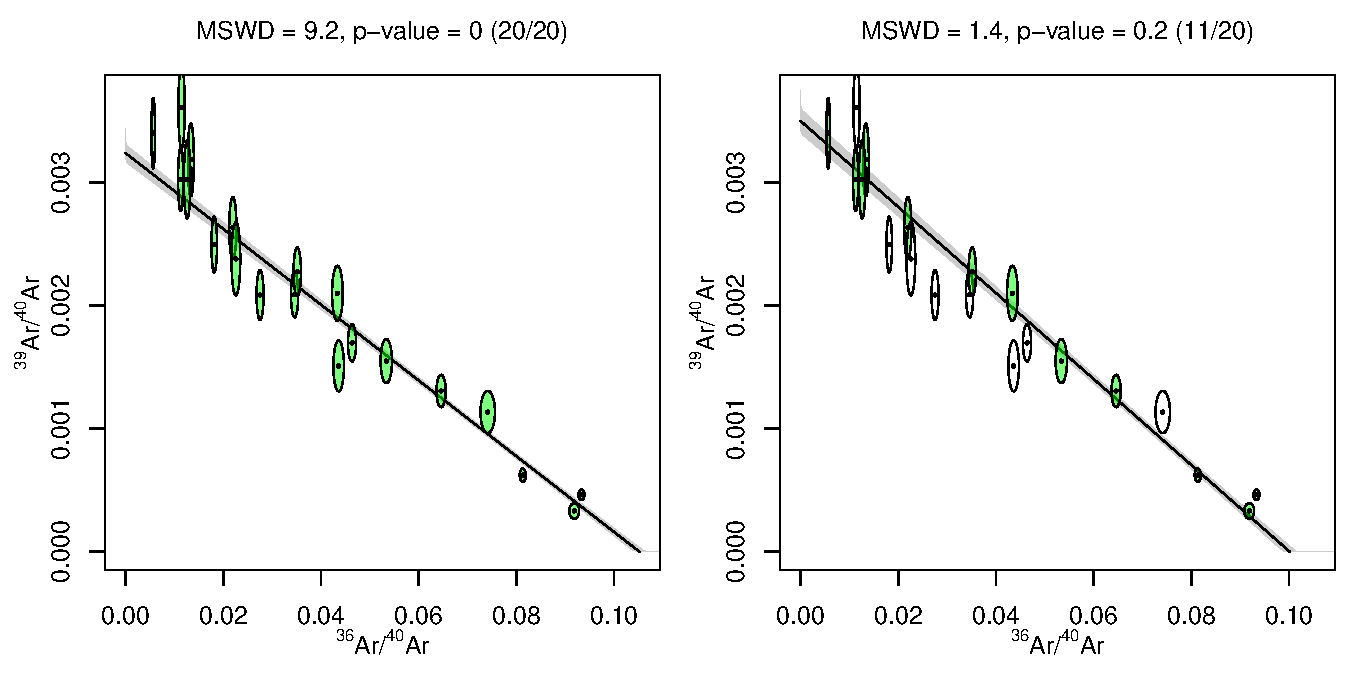
\includegraphics[width=\linewidth]{../figures/isochron.pdf}
\end{minipage}
\begin{minipage}[t][][t]{.3\linewidth}
  \captionof{figure}{Synthetic
    \textsuperscript{40}Ar--\textsuperscript{39}Ar dataset (a) without
    and (b) with `outlier' removal. The data are generated from a true
    isochron with horizontal intercept $x_0=0.1$ and a vertical
    intercept $y_0=1/298.5$. Excess dispersion was added to both the
    \textsuperscript{36}Ar/\textsuperscript{40}Ar (10\%) and
    \textsuperscript{39}Ar/\textsuperscript{40}Ar (5\%) ratios.}
  \label{fig:synthetic_Ar-Ar}
\end{minipage}

\subsection{Concordia ages}\label{sec:concordia}

The U--Pb method comprises two independent chronometers based on the
radioactive decay of two isotopes of uranium (\textsuperscript{238}U
and \textsuperscript{235}U) to two lead isotopes
(\textsuperscript{206}Pb and \textsuperscript{207}Pb, respectively),
providing an internal quality control mechanism that is absent from
most other geochronometers. Concordance of the two clocks can be
tested using a chi-squared statistic:

\begin{equation}
  \chi^2 =
  \left[
    \begin{array}{@{}c@{}}
      X - \left(e^{\lambda_{235}t_c} - 1\right) \\
      Y - \left(e^{\lambda_{238}t_c} - 1\right)
    \end{array}
    \right]^T
  \left[
    \begin{array}{@{}cc@{}}
      s[X]^2 & s[X,Y] \\
      s[X,Y] & s[Y]^2
    \end{array}
    \right]^{-1}
  \left[
    \begin{array}{@{}c@{}}
      X - \left(e^{\lambda_{235}t_c} - 1\right) \\
      Y - \left(e^{\lambda_{238}t_c} - 1\right)
    \end{array}
    \right]
  \label{eq:concordance}
\end{equation}

\noindent where $X$ and $Y$ are the measured
\textsuperscript{207}Pb/\textsuperscript{235}U and
\textsuperscript{206}Pb/\textsuperscript{238}U ratios; $s[X]^2$,
$s[Y]^2$ and $s[X,Y]$ their (co)variances; and $t_c$ is the `concordia
age', which is obtained by minimising $\chi^2$. If the age is
perfectly concordant and analytical uncertainty is the only source of
scatter, then $\chi^2$ follows a chi-squared distribution with $\nu =
1$ degree of freedom \citep{ludwig1998}.\medskip

Laser ablation inductively coupled plasma mass spectrometry
(LA-ICP-MS) is a widely used technique for in-situ U--Pb
geochronology. It produces raw instrument data consisting of time
series of \textsuperscript{206}Pb, \textsuperscript{207}Pb, and
\textsuperscript{238}U measurements (in V, A, or Hz), which comprise
two components: the `background', measured before laser ablation, and
the `signal', measured during laser ablation. A key step in the data
reduction process is the definition of `selection windows' that group
`stable' segments of the mass spectrometer signal. Some data reduction
packages support this process by providing an interactive `live
concordia' diagram, in which the effect of the selection window on the
inferred U--Pb composition is immediately visible
\citep[e.g.,][]{petrus2012}. Although such interactive user interfaces
can be helpful, they also introduce a mechanism for generating
isotopic compositions that are `too good to be true'
(Figure~\ref{fig:concordia}).\medskip

\noindent\begin{minipage}[t][][b]{.7\linewidth}
  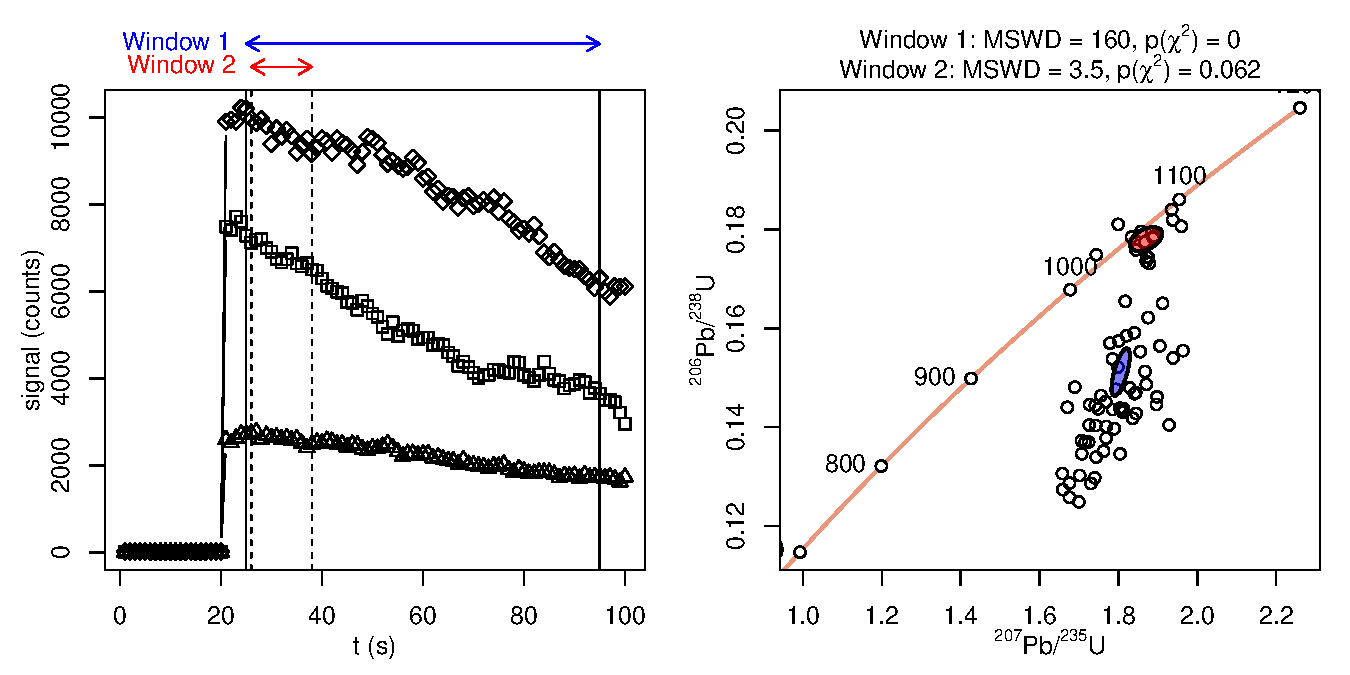
\includegraphics[width=\linewidth]{../figures/concordia.pdf}
\end{minipage}
\begin{minipage}[t][][t]{.3\linewidth}
  \captionof{figure}{a) synthetic time-resolved LA-ICP-MS dataset
    showing \textsuperscript{238}U (diamonds), \textsuperscript{206}Pb
    (squares) and \textsuperscript{207}Pb (triangles), and two
    selection windows; b) `live' concordia diagram of the individual
    mass spectrometer signals, with the means of the integrations for
    the two selection windows shown as blue and red ellipses,
    respectively.}
  \label{fig:concordia}
\end{minipage}

\subsection{Mixtures of over- and under-dispersed datasets}
\label{sec:mixtures}

Having reviewed some key mechanisms that may result in underdispersion
on the sample level, this section will consider their effect on a
collection of multiple samples. Let us first consider the simplest
case of a collection of `perfect' samples, which exhibit no
overdispersion whatsoever.\medskip

For fission track data and weighted means, `perfection' means that all
the analysed grains have exactly the same age, with the scatter of the
dates being exclusively caused by analytical uncertainty. For
isochrons, `perfect' data mean that the true (but unknowable) isotopic
ratios fall exactly on an isochron, with the scatter of the measured
isotopic ratio estimate being only caused by analytical uncertainty
\citep{kalsbeek1992}. Finally, for concordia age calculation, the true
(but unknown) \textsuperscript{207}Pb/\textsuperscript{235}U and
\textsuperscript{206}Pb/\textsuperscript{238}U ratios fall exactly on
the Wetherill concordia line, and the dispersion of the measured
\textsuperscript{207}Pb/\textsuperscript{235}U and
\textsuperscript{206}Pb/\textsuperscript{238}U ratio estimates is due
to analytical uncertainty alone. For a collection of such `perfect'
samples (for all of which $H_0$ is true), the ECDF of a random
selection of p-values would stradddle the 1:1 line. Therefore, on
average 5\% of the sample would erroneously be labelled as being
overdispersed when in fact they are not, resulting in a Type~I
error.\medskip

The outlier rejection procedures outlined in
Sections~\ref{sec:synthetic-FT}--\ref{sec:concordia} reduce the
proportion of Type~I errors to zero, causing the ECDF of the p-values
to shift to the right and slightly below the 1:1 line (blue
in Figure~\ref{fig:synthetic_ecdfs}a). This can be referred to as
`mild' underdispersion. More extreme degrees of underdispersion
require that the p-value cutoff is raised from the usual value of
$\alpha = 0.05$ to higher values (e.g., $\alpha=0.5$). Alternatively
(and equivalently), more extreme degrees of underdispersion can also
arise from the use of MSWDs instead of p-values to identify
`outliers'.\medskip

Although there is a one-to-one mapping between MSWD and p-value, this
mapping changes as a function of sample size. Suppose that a
collection of unequally sized samples was culled until
MSWD\,$\leq$\,1. Then this MSWD-cutoff would be equivalent to
$\alpha=0.59$ for $n=5$, to $\alpha=0.54$ for $n=20$ and $\alpha=0.51$
for $n=100$. The p-value distribution for these extreme levels of
outlier rejection would fall further below the 1:1 line, providing the
diagnostic signature of `severe' underdispersion
(red in Figure~\ref{fig:synthetic_ecdfs}a).\medskip

Having considered the effect of outlier rejection on `perfect'
samples, let us now move on to more realistic scenarios that exhibit
some degree of overdispersion. Without outlier rejection, the p-value
distribution of such an `imperfect' collection of studies would fall
completely above and to the left of the 1:1 line. Depending on the
severity of the overdispersion, there may or may not be any p-values
exceeding $\alpha=0.05$. If all the samples in the collection were
overdispersed (so that all $H_0$ are false), then any p-value
exceeding $\alpha$ would constitute a Type~II error (false
negative). Subjecting the overdispersed collection of samples to
outlier rejection shifts the p-value distribution to the right and
below the 1:1 line, greatly increasing the number of Type~II errors
(blue and red in Figure~\ref{fig:synthetic_ecdfs}b).\medskip

Finally, let us consider the most realistic scenario, in which a
collection of multiple samples, exhibiting different degrees of
overdispersion, either have or have not been subjected to outlier
rejection. The resulting p-value distribution of such a mixture would
consist of a steep segment of low p-values obtained from samples that
have not undergone outlier removal, followed by a convex-upward
segment marking examples that have undergone outlier removal.  An
important observation is that only extreme levels of outlier removal
manage to push the p-value distribution below the 1:1 line
(orange in Figure~\ref{fig:synthetic_ecdfs}b).

\noindent\begin{minipage}[t][][b]{.7\linewidth}
  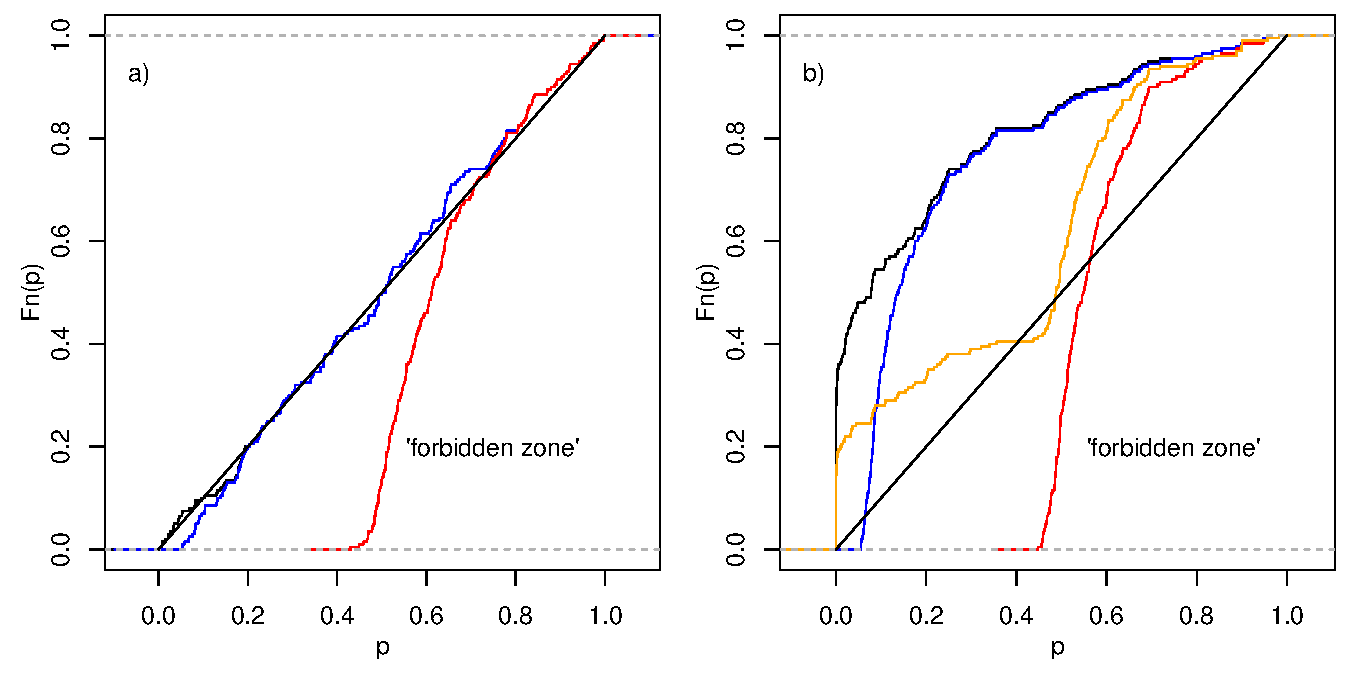
\includegraphics[width=\linewidth]{../figures/synthetic_ecdfs.pdf}
\end{minipage}
\begin{minipage}[t][][t]{.3\linewidth}
  \captionof{figure}{p-value distributions for a) a non-dispersed
    (`perfect') collection of samples; and b) a collection of samples
    that exhibit up to 2\% overdispersion.  Black curves mark p-value
    distributions without outlier removal; blue functions mark
    distributions with outlier removal using an $\alpha\geq{0.05}$
    p-value cutoff; and red curves with an MSWD\,$\leq$\,1 cutoff. The
    orange function is a 50/50 mixture of the black and the red
    distribution.}
  \label{fig:synthetic_ecdfs}
\end{minipage}

\section{Natural examples}\label{sec:real}

Section~\ref{sec:synthetic} reviewed the principal mechanisms that may
cause underdispersion in geochronology, using synthetic examples.
Section~\ref{sec:mixtures} showed that, in extreme cases, excessive
outlier rejection may cause the p-value distribution of a collection
of multiple studies to fall below the 1:1 line and in the `forbidden
zone'. This Section will investigate whether such excessive outlier
rejection occurs in real datasets. It is important to reiterate that,
the most extreme cases nothwithstanding (MSWD$ = 0$, $p = 1$), it is
generally not possible to identify with certainty that any given
sample is `too good to be true'. However, a clearer picture emerges
when considering multiple studies together. The purpose of this
meta-analysis is not to point fingers at individual researchers. As
explained in the previous sections, outlier rejection is often done
for good reasons and many cases of underdispersion may be
unintentional.

\subsection{Fission tracks}\label{sec:FT}

Fission track analysis is especially well suited to detect cherry
picking, for two reasons.  First, error propagation of fission track
data (using the external detector method) is so straightforward
\citep{green1981b} that cherry picking is the sole mechanism that can
push the p-value distribution into the `forbidden zone'
(Section~\ref{sec:synthetic-FT}).  Second, unlike most other
geochronometers (which are based on isotopic ratio estimates obtained
by mass spectrometry), fission track analysis is based on manual
counts of damage tracks under an optical microscope. This manual
process is particularly prone to observer bias \citep{tamer2025},
providing a particularly compelling reason to investigate fission
track data for underdispersion.\medskip

A useful `baseline result' is provided by a dataset of 176 p-values
for fission track reference materials analysed by \cite{iwano2018}. By
definition, reference materials are expected to exhibit little or no
overdispersion. However, in reality even these `ideal' materials are
shifted towards low p-values compared to the uniform distribution
(Figure~\ref{fig:Iwano}). This confirms that overdispersion is the
rule rather than the exception in nature.  If even geochronological
reference materials exhibit (mild) overdispersion, then the p-values
of `real' samples --with all their natural complexity-- should
definitely be prohibited from plotting below the 1:1 line in
ECDF-space.  However, a compilation of fission track analyses from the
\texttt{geochron.org} database indicates otherwise.\medskip

At the time of writing, \texttt{geochron.org} contained 434 fission
track samples, 201 of which reported p-values. All these samples used
the external detector method \citep{hurford1983}, whose error
propagation is straightforward \citep{green1981b} and standardised.
Instead of plotting towards the left of \citet{iwano2018}'s p-value
distribution, the \texttt{geochron.org} data plot nearly completely to
the right of the reference materials (Figure~\ref{fig:Iwano}). One
third of the p-values plot in the `forbidden zone'. This means that
one third of the fission track samples in the \texttt{geochron.org}
database are too good to be true.

\noindent\begin{minipage}[t][][b]{.4\linewidth}
  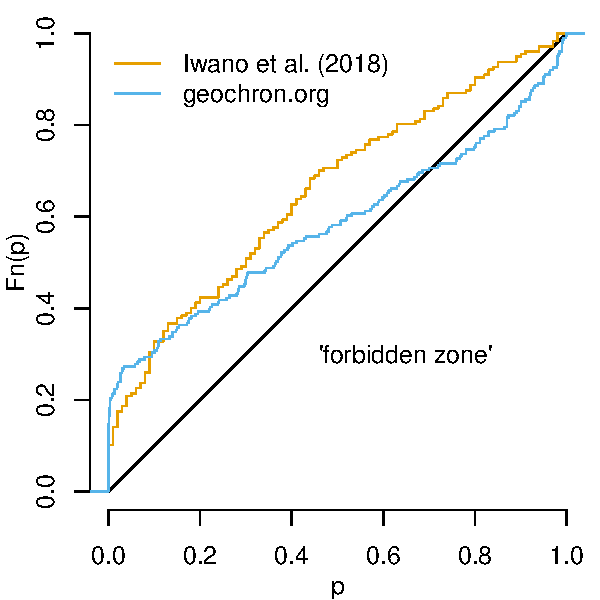
\includegraphics[width=\linewidth]{../figures/Iwano.pdf}
\end{minipage}
\begin{minipage}[t][][t]{.6\linewidth}
  \captionof{figure}{The red curve represents a fission track dataset
    of reference materials \citep{iwano2018}, which shows no
    detectable evidence for cherry picking. In contrast, the blue curve
    corresponds to a compilation of fission track data in which 30\% of
    the p-values are underdispersed to such a degree that they are
    `too good to be true'.}
  \label{fig:Iwano}
\end{minipage}

\subsection{A compilation of Nature papers}

The second real-world underdispersion study will investigate
mass-spectrometer based geochronology data, including U--Pb,
\textsuperscript{40}Ar/\textsuperscript{39}Ar, Rb--Sr and other
methods.  Whereas outlier rejection of fission track data nearly
always done by p-value, other geochronometers generally use the MSWD
to guide data selection. Because the acronym `MSWD' is exclusively
used in geochronology (with other fields of science referring to the
statistic as the `reduced chi-squared statistic'), it is easy to
extract measures of geochronological dispersion from the scientic
literature. Recall that, as a rule-of-thumb, $\mbox{MSWD}\approx{1}$
indicates that a model is a `good' fit for the data, whilst
$\mbox{MSWD}\gg{1}$ indicates that the data are overdispersed with
respect to the analytical uncertainties and $\mbox{MSWD}\approx{0}$
indicates underdispersed (and possibly cherry picked)
datasets.\medskip

A database of 100 high profile geochronological papers was compiled
with the aptly named `Publish or Perish' software \citep{harzing2010},
using `MSWD' as the sole keyword, and `Nature' as the target journal.
The search was restricted to Nature journals (including Nature, Nature
Geoscience, Nature Communications and Scientific Reports) for two
reasons. First, they are the most `impactful' publications, which
should be held to the highest standards. Second, Nature publications
provide consistently rich supplementary data archives. These are
necessary to recover the degrees of freedom of the MSWD-statistics,
which are needed to compute the corresponding p-value. Some papers
report two p-values per sample, one for the complete dataset, and one
for the `cleaned' data with `outliers' removed. For these cases both
values were included in the database.
\medskip

The 100 publications contained 650 MSWD-values, 36.3\% of which are
less than one. The ECDF of the corresponding p-values is shown in
black on Figure~\ref{fig:ECDF}b. Only the bottom 85\% of this curve
plots above the 1:1 line. The remaining 15\% of the p-value
distribution falls in the forbidden zone of impossibly good
results. 9\% of the p-values exceed 0.95. As mentioned before, there
are two possible causes for this pattern.  One possibility is
incorrect error propagation. Mass spectrometer data processing is
complex and it is certainly possible that some uncertainties in the
geochronological literature have been overestimated. For example, this
could happen by failure to distinguish between systematic and random
sources of uncertainty \citep{renne1998}.  A second possible cause of
underdispersion is excessive outlier rejection.\medskip

To distinguish between the two causes of underdispersion, it is useful
to group the p-values for different chronometers. Note that the Nature
compilation does not contain any fission track data. The two largest
groups are U--Pb (320 p-values) and Ar--Ar (119 p-values).  Both have
ECDFs with similar proportions of analyses falling in the forbidden
zone, at 21\% and 18.5\% respectively. It seems unlikely that the data
reduction software for both methods (which use different types of mass
spectrometers) would be equally flawed. It is therefore also unlikely
that incorrect error propagation is the sole cause of
underdispersion. Excessive outlier rejection is a more likely
culprit. This conclusion is corroborated by grouping the collection of
p-values according to the statistical method of analysis.\medskip

Isochrons exhibit the lowest percentage of p-values in the forbidden
zone, at 11\% (out of 223 p-values).  This increases to 15\% for
weighted means (316 p-values) and 20\% for
\textsuperscript{40}Ar/\textsuperscript{39}Ar plateaux (80 p-values).
It is not surprising that the latter exhibit the strongest evidence
for underdispersion, as the definition of a
\textsuperscript{40}Ar/\textsuperscript{39}Ar plateau involves
selecting measurements that overlap within analytical uncertainty
\citep{dalrymple1969,jourdan2009}. Plateaux are, therefore, `cherry
picked' by definition.

\noindent\begin{minipage}[t][][b]{.7\linewidth}
  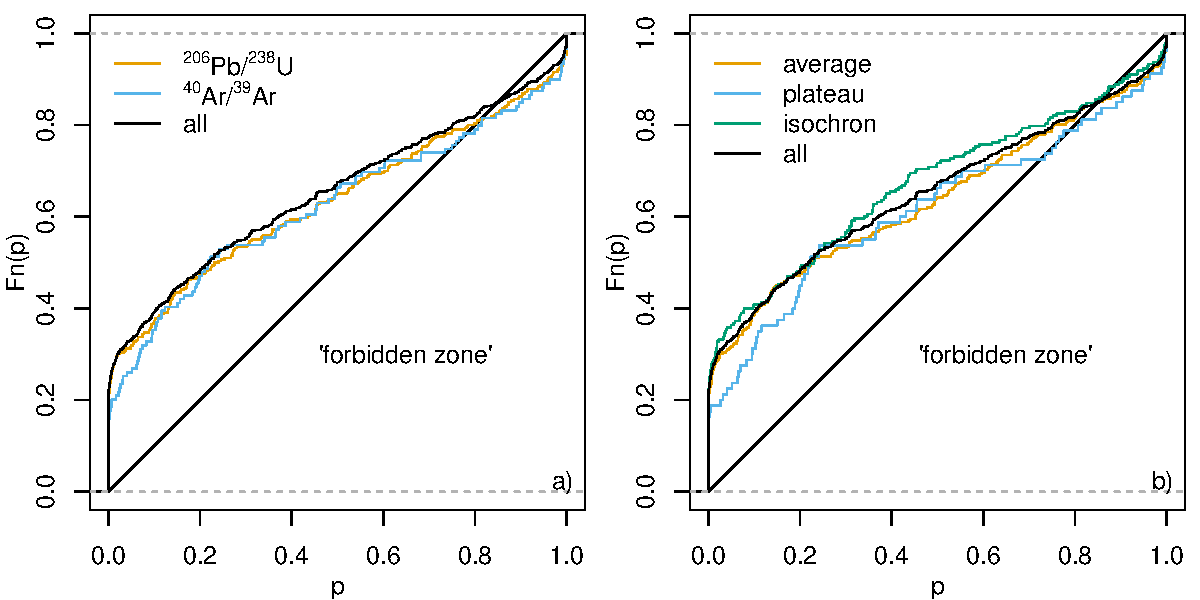
\includegraphics[width=\linewidth]{../figures/Nature.pdf}
\end{minipage}
\begin{minipage}[t][][t]{.3\linewidth}
  \captionof{figure}{p-value distributions for the compilation of 100
    Nature papers. The black curves represent the full dataset of 650
    p-values. The colours group the dataset according to the
    geochronometer (a) and plotting device (b).  }
  \label{fig:Nature}
\end{minipage}

\subsection{The Geologic Time Scale (GTS2020)}\label{sec:GTS2020}

The Geologic Time Scale (GTS) is a standardised framework that
organises Earth's ca.\,4.56 billion-year history into a coherent
timeline, enabling scientists to correlate rock records and place
geological, climatic, and biological events in chronological order. It
originated in the 18\textsuperscript{th}--19\textsuperscript{th}
centuries as a relative system based on biostratigraphy. In the
20\textsuperscript{th} century, the development of radiometric dating
transformed the GTS into a calibrated system that integrates relative
stratigraphy with absolute numerical ages, allowing increasingly
precise timing of events \citep{holmes1947}.\medskip

Over time, international efforts, particularly through the
International Commission on Stratigraphy, have standardized boundaries
using globally agreed reference points (Global Boundary Stratotype
Sections and Points -- GSSPs) and continually refined the scale as new
data emerge. The latest synthesis, GTS2020, incorporates advances in
geochronology, astrochronology, and stratigraphic correlation to
produce a more precise and highly resolved timeline
\citep{gradstein2020, schmitz2020}.\medskip

The GTS places great emphasis on analytical precision. However,
accuracy is equally if not more important. Because accuracy and
precision can be competing targets (`bias-variance tradeof'), the
p-value distribution of the GTS is of particular interest. The
geochronological database underlying GTS2020 contains 407 entries.  It
was not possible to obtain p-values for all these entries because (1)
some dates were derived from unpublished sources; (2) other dates were
locked behind unscaleable pay walls; and (3) seventeen age constraints
were based on single grain analyses, for which it is not possible to
calculate an MSWD\footnote{Note that selecting a single analysis out
of a collection of multiple measurements could be considered the
ultimate degree of cherry picking. However, single grain analyses were
omitted from this study, resulting in a conservative (optimisitic)
picture of outlier rejection.}. Nevertheless, going back to the
original publications cited in the GTS2020 database did yield 355
MSWD-values and sample sizes, from which 355 p-values were
calculated.\medskip

The overall distribution plots close to the 1:1 line, reflecting the
GTS committee's best effort to identify discrete age components that are
consistent within the analytical uncertainties. Nevertheless, 25\% of
the age constraints plot slightly below the 1:1 line, including 5\% of
the U--Pb data and 90\% of the Ar--Ar data (Figure~\ref{fig:GTS}).

\noindent\begin{minipage}[t][][b]{.4\linewidth}
  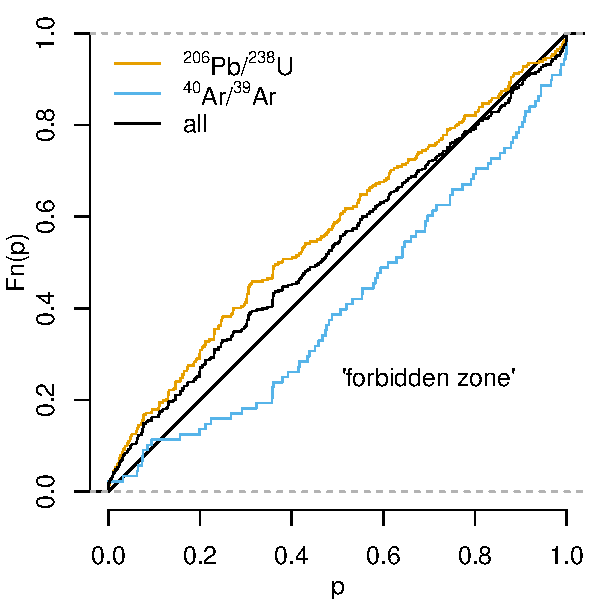
\includegraphics[width=\linewidth]{../figures/GTS.pdf}
\end{minipage}
\begin{minipage}[t][][t]{.6\linewidth}
  \captionof{figure}{p-value distribution of the Geologic Time Scale
    \citep[GTS2020,][]{gradstein2020}. The full dataset of 355 age
    constraints is shown in black; colours mark the sub-populations of
    \textsuperscript{40}Ar/\textsuperscript{39}Ar (88 p-values) and
    \textsuperscript{206}Pb/\textsuperscript{238}U (328 p-values)
    data.}
  \label{fig:GTS}
\end{minipage}

\subsection{Detrital zircon U--Pb geochronology}\label{sec:detrital}

All the p-value distributions presented thus far were extracted from
collections of multiple studies, representing dozens of samples. This
was necessary because most geochronological uses of the chi-squared
test evaluate the consistency between aliquots of the same
sample. Therefore, each sample corresponds to one MSWD value and,
hence, one p-value.  The single-grain concordia age calculation
procedure of Section~\ref{sec:concordia} is an exception to this rule.
It tests the agreement between the
\textsuperscript{206}Pb/\textsuperscript{238}U and
\textsuperscript{207}Pb/\textsuperscript{235}U clocks \emph{within}
each aliquot. Therefore, a single detrital zircon U--Pb sample can
produce an entire p-value distribution.\medskip

As explained in Section~\ref{sec:concordia}, modern LA-ICP-MS data
reduction software allows geochronogists to `optimise' their choice of
selection windows using a `live concordia' diagram, providing a
mechanism to generate underdispersed datsets. A literature review has
revealed some examples of this in published datasets. However,
presenting those datasets here would single out individual
researchers. This is not the purpose of the current study, which seeks
to evaluate the occurrence of underdispersion in geochronology as a
whole. Therefore, the inappropriate use of `live isochrons' will not
be illustrated with a published dataset, but with a new one.\medskip

Figure~\ref{fig:Droellner} presents a dataset of 150 zircon U--Pb
measurements for an inter-laboratory comparison sample prepared by
Dr. Maximilian Dr\"{o}lner (University of G\"{o}ttingen). The full
results of the comparison study will be presented in a forthcoming
publication. Its details are irrelevant for the purpose of the present
investigation, which merely aims to quantify the dispersion of the
data.\medskip

The sample was analysed at University College London using an Agilent
7900 ICP-MS coupled to a New Wave NWR193 excimer laser, operated at
10\,Hz with a spot size of 25\,\textmu{m}, using a 5\,s warmup time,
followed by 25\,s of ablation and 5\,s of washout.  Data reduction was
performed with \texttt{KJ} \citep{vermeesch2026b}, using
Ple{\v{s}}ovice and 91500 zircon \citep{slama2008,wiedenbeck1995} as 
primary reference materials and GJ-1 \citep{jackson2004} as a
secondary standard. Raw data and FAIR data reduction procedures are
provided in the supplementary information.\medskip

The blue error ellipses in Figure~\ref{fig:Droellner}a) show the
results obtained using \texttt{KJ}'s default selection windows,
without manual adjustment and presented as a Wetherill concordia
diagram generated in \texttt{IsoplotR}~7.0 \citep{vermeesch2018c}.
The blue ellipses show the same sample after `optimal' signal window
adjustment, which was achieved by exploring all continuous sections of
the signal of at least 50 integrations long, and selecting the window
yielding the lowest MSWD using the definition of
Equation~\ref{eq:concordance}. Unsurprisingly, this extreme example of
cherry picking results in a p-value distribution in which nearly 90\%
of the 150 grains are `too good to be true'.

\noindent\begin{minipage}[t][][b]{.7\linewidth}
  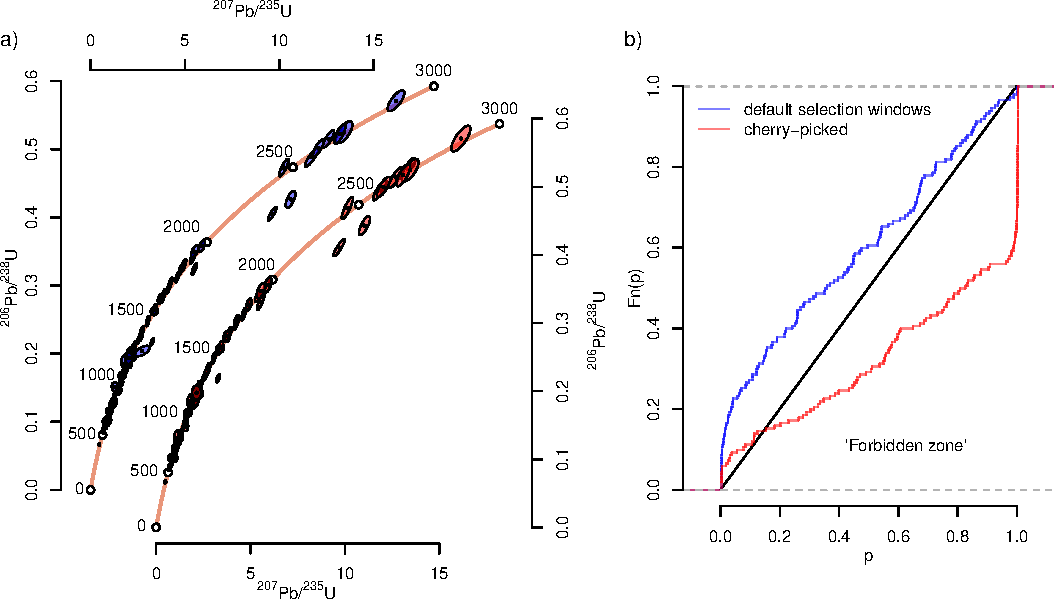
\includegraphics[width=\linewidth]{../figures/Droellner.pdf}
\end{minipage}
\begin{minipage}[t][][t]{.3\linewidth}
  \captionof{figure}{a) Wetherill concordia diagrams for a detrital
    zircon U--Pb dataset acquired by LA-ICP-MS without (blue) and
    with (red) the `optimal' window selection approach of
    Section~\ref{sec:concordia}. b) the corresponding p-value
    distributions.}
  \label{fig:Droellner}
\end{minipage}

\section{Discussion: (why) does underdispersion matter?}

There are many mechanisms that can produce overdispersed datasets. In
fact, a case could be made that overdispersion should be the rule
rather than the exception \citep{kalsbeek1992,vermeesch2025c}.  In
comparison, it is not so easy to explain underdispersion.  Excessive
outlier detection is the most likely culprit behind the
underdispersion observed in all the case studies of
Section~\ref{sec:real}.\medskip

The synthetic examples of Section~\ref{sec:mixtures} showed that, in a
meta-analysis that combines overdispersed datasets with underdispersed
ones, it is not easy to pull the p-value distribution into the
`forbidden zone'.  Doing so requires extremely levels of outlier
rejection. All the case studies presented in this paper show evidence
for such extreme outlier rejection in at least some of the
samples.\medskip

For example, the fact that one third of the fission track data plot
below the 1:1 line of the p-value distribution plot indicates that
\emph{at least} one third of the fission track samples have been
cherry picked to a degree that cannot be explained by the `observer
drift' phenomenon of Section~\ref{sec:synthetic-FT}.  And the fact
that 90\% of the Ar--Ar data in the GTS plot in the `forbidden zone'
suggests that geochronologists apply more aggressive outlier rejection
criteria than the 5\% p-value cutoff advocated by
\citet{jourdan2009}. It appears that at least some analysts aim to
push the p-values of their data as close to unity as possible.  This
reflects a fundamental misunderstanding of practice of statistical
hypothesis testing.\medskip

Whilst the evidence for excessive outlier rejection is clear, one
might ask the question: ``does it make a difference?''. After all,
Mendel's data were almost certainly cherry picked, yet the scientific
conclusion draw from them remains correct. Does the same phenomenon
apply to geochronology? There are four answers to this
question.\medskip

First, it should be emphasized that the burden of proof should not
rest with those who identify underdispersion to demonstrate its
importance. Rather, it should lie with those who apply excessive
outlier rejection to show that the underdispersion does \emph{not}
matter. It may be true that eliminating underdispersion would not
change the scientific conclusions of most studies. However, the
possibility that it could affect the conclusions of \emph{some}
studies is concerning. Moreover, in cases where excessive outlier
rejection does not alter the conclusions, one could argue that such
rejection serves no meaningful purpose.\medskip

Second it is important to point out a fundamental difference between
Mendel's pea experiment and the geochronological context. Mendel's pea
experiment ---and \citet{fisher1936}'s reanalysis--- tested a `natural'
binary hypothesis, aiming to find out if selected traits of peas are
random or inherited.  Prior to the experiment, there was a real
probability that the null hypothesis (random allocation of traits) was
true. In contrast, the geochronological null hypothesis (the data are
perfectly homogeneous) cannot be true

\citep{vermeesch2025c}. Therefore, the purpose of geochronological
chi-squared tests is not to test \emph{if} the data are overdispersed,
but to test whether the overdispersion is \emph{statistically
significant}. In statistical terms, the probability of committing a
Type~I error was 5\% for Mendel's experiment, and 0\% for
geochronological experiments. Consequently, the probability of
committing a Type~II error is much higher for geochronological
datasets then for Mendel's pea data.\medskip

Third, attention should be drawn to the important phenomenon of the
`bias-variance' tradeof in mathematical statistics. When estimating a
numerical quantity such as the mean, slope or intercept of a
collection of measurements, statistical precision (`variance') and
accuracy (`bias') tend to be competing goals. A classic example is the
Bessel correction of the sample standard deviation. Given a collection
of $n$ measurements $\{x_1,\ldots,x_n\}$ drawn from a normal
distribution with mean $\mu$ and standard deviation $\sigma$, the mean
can be estimated as $\hat{\mu} = \sum_{i=1}^n x_i$ and the standard
deviation as $\hat{\sigma} = \sum_{i=1}^{n}(x_i-\mu)^2/n$ if $\mu$ is
known, \emph{or} as $\hat{\sigma} =
\sum_{i=1}^{n}(x_i-\hat{\mu})^2/(n-1)$ if $\mu$ is unknown. The
denominator $n-1$ in the latter case inflates the variance (and hence
reduces its precision) but reduces the bias (and increases the
accuracy) of the estimate for $\sigma$.\medskip

Underdispersion creates the opposite situation, whereby excessive
outlier rejection artificially improves precision at the expense of
accuracy. This is particularly pertinent for the Geologic Time Scale.
As reviewed in Section~\ref{sec:GTS2020}, great efforts are made to
improve the precision of the chronostratigraphic calibration that
underlies the GTS. It would be most unfortunate if this focus on
precision came at the expense of accuracy, which is arguably more
important. When accuracy is not guaranteed, precision loses its
meaning. Fortunately, the overall degree of overdispersion of the GTS
is small compared to the other case studies. Nevertheless, the
underdispersion of the Ar--Ar data is concerning.\medskip

Fourth, when data appear too good to be true, it suggests that valid
measurements have been improperly excluded, leading to the loss of
potentially valuable information. Overdispersion can reflect processes
such as magma residence times \citep{rioux2012} or cooling rates
during tectonic exhumation \citep{galbraith1993}. Thanks to advances
in mass spectrometry, geochronologists are increasingly capable of
detecting such subtle complexities
\citep{phillips2013}. Overdispersion is not a flaw to be eliminated
but a feature to be measured and interpreted
\citep{kalsbeek1992,vermeesch2025c}. Excessive outlier rejection
discards all this information, representing an opportunity cost for
scientific discovery.

\section{Conclusions}

This paper has introduced a new graphical method to detect
underdispersion in collections of geochronological data.  The
distribution of the p-values for sample homogeneity may be negatively
skewed with respect to a uniform distribution but must not be
positively skewed. The area below the 1:1 line of a cumulative
distribution plot marks a `forbidden zone', reflecting the presence of
samples whose internal constency is unrealistically good.\medskip

Underdispersion can arise from incorrect error propagation, or from
overzealous outlier rejection. Application of the p-value method to
synthetic and real datasets shows that it affects all
geochronometers. Underdispersion is particularly common in fission
track analysis and \textsuperscript{40}Ar/\textsuperscript{39}Ar age
plateaux.  For these cases, the degree of underdispersion is too great
to be explained by faulty error propagation or mild outlier
rejection. To consistently push substantial segments of the p-value
distribution into the `forbidden zone' requires extreme levels of
outlier rejection in which researchers actively aim to push their MSWD
to zero.\medskip

This study has not made an attempt to assess if the observed
underdispersion has led to incorrect scientific conclusions. Doing so
would require highlighting specific underdispersed studies, which
could be perceived as pointed criticism at specific authors.  As
explained in Section~\ref{sec:real}, that is not the intention of this
study.\medskip

In the case of the Geologic Time Scale, underdispersion has two
negative effects. First, it leads to unrealistic uncertainty
estimates, giving geochronologists false confidence in the
chronostratigraphy.  Second, and more importantly, the inflated
precision comes at the cost of reduced accuracy. The magnitude of this
problem varies across the timescale, depending on the degree of
underdispersion of the underlying geochronological datasets.\medskip

Some of the underdispersed datasets in the GTS are old and predate the
increased awareness of overdispersion as a fact of life, rather than a
nuisance to be removed by outlier rejection. However, these old
studies have a lasting effect on the practice of geochronology.
Extreme levels of outlier rejection persist in modern time scale
studies because modern datasets are expected to have better age
precision than old datasets. To break out of this self-perpetuating
situation, it is important to recognise that the precision of some age
boundaries is not limited by analytical uncertainty, but by geological
complexity. Therefore, geochronologists should not be afraid to update
GTS tie points with new data that are less precise (but more
accurate).\medskip

Going forward, the p-value distribution can be used to help
geochronologists identify when outlier rejection has gone too far.  An
even better solution would be to abandon the misconception that
overdispersion is inherently `bad'.  Overdispersed datasets are more
likely to be rejected during peer review than tightly clustered ones,
which directly and indirectly promotes underdispersion.  Poorly
informed reviewers may reject such datasets outright, skewing the
literature toward high p-values \citep[publication
  bias,][]{ioannidis2005}.  In turn, the difficulty of publishing low
p-value results incentivises aggressive outlier rejection.  Peer
pressure to produce `perfect' data may partially or completely explain
the prevalence of underdispersed geochronology data in high profile
publications such as Nature.\medskip

In the case of LA-ICP-MS signal window selection, outlier rejection
occurs in early stages of the data processing pipeline, before the
isotopic ratios are calculated. Unless the raw mass spectrometer data
of such data are shared, it is impossible to undo this source of
underdispersion. Fixing this problem will require the adoption of FAIR
(Findable, Accessible, Interoperable, and Reusable) data processing
pipelines \citep{wilkinson2016}.  Currently, geochronological results
are typically reported as small tables of processed isotopic ratios
and uncertainties. The raw mass spectrometer data and complete data
processing algorithms used to derive these results are rarely
shared. This lack of transparency creates opportunities for
underdispersion.  A new generation of data reduction software such as
\texttt{geochron@home} \citep{vermeesch2026} and \texttt{KJ}
\citep{vermeesch2026b} show that this is possible.

\section*{Appendix: Type~I and Type~II cherry picking}

Two types of cherry picking can be distinguished, each aligned with
one side of the significance dichotomy and named by analogy with
related concepts in mathematical statistics. Type~I cherry picking
involves selecting data that contradict a pre-defined
hypothesis. Type~II cherry picking selects data that support a
hypothesis.\medskip

As a concrete example of Type~I cherry picking,
consider a multivariate dataset (e.g., the concentration of $N$
chemical species in $M$ samples). It is common practice in exploratory
data analysis to plot all pairs of variables against each other in an
$N\times{M}$ grid of scatter plots. When doing this it is inevitable
that some of these pairs exhibit a statistically significant
correlation.\medskip

Figure~\ref{fig:type1} shows 18 pairs of data, drawn from a random
uniform population with no correlation.  Hence, the correlation
coefficient of the population ($\rho$) is zero.  However, the estimated
correlation coefficient of the data ($r$) is not. It varies between
$-1$ and $+1$ as a result of random sampling variability.  The degree
of correlation can be formally evaluated by formulating a test
statistic $t \equiv r\sqrt{n-2}/\sqrt{1-r^2}$.  We can then formulate
the following hypotheses:

\begin{description}
\item{$H_0$:} $x$ and $y$ are independent ($\rho = 0$)
\item{$H_a$:} $x$ and $y$ are correlated ($\rho \neq 0$)
\end{description}

$H_0$ is true for the synthetic example, and any rejection of this
hypothesis constitutes a Type~I error. The probability of incurring
such an error is defined by the significance cutoff $\alpha$. However,
Section~\ref{sec:ecdf} showed that the probability of committing a
Type~I error increases to $1 - (1 - \alpha)^n$ when the number of
tests is increased from 1 to $n$. When $n>14$, the probability of
committing a Type~I error exceeds that of not committing one.\medskip

Failure or refusal to account for this phenomenon is sometimes
referred to as `p-hacking' or `data dredging'. Because it increases
the probability of committing a Type~I error, this paper labels the
phenomenon as `Type~I cherry picking', to emphasise the difference
with the geochronologicaly context, in which data are not manipulated
to lower the p-value, but to boost it.\medskip

The occurrence of Type~I cherry picking is difficult to prove. It
requires repeating the entire experiment to verify if the same result
is obtained.  Type~II cherry picking is easier to detect, and
radiometric geochronology is uniquely suited for this purpose. Unlike
other research fields (such as genetics, say) it offers no incentives
for Type~I cherry picking, but ample opportunities for Type~II cherry
picking (Section~\ref{sec:synthetic}).  This paper promotes the
cumulative distribution of the p-values as a graphical device to
identify the problem.\medskip

\noindent
\includegraphics[width=\textwidth]{../figures/type1.pdf}
\captionof{figure}{18 scatter plots of bivariate random uniform data,
  with indication of the coefficient of determination ($r^2$) and the
  p-value for correlation. The one `significant' result (p-value =
  0.00063) is a Type~I error.}
\label{fig:type1}

\section*{Acknowledgments}

This research has been supported by the Natural Environment Research
Council (grant no. NE/T001518/1). The author would like to thank Blair
Schoene and Dan Condon for reviewing an earlier submission, and Murat
Tamer for encouragement.

\bibliographystyle{abbrvplainnat}
\bibliography{biblio.bib}

\end{document}
